\usetikzlibrary{shapes,arrows,calc,decorations.markings}


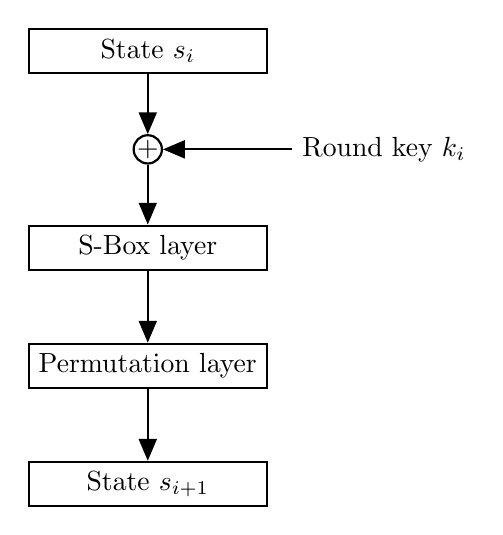
\begin{tikzpicture}
[
auto, thick, >=triangle 45,
block/.style    = {draw, thick, rectangle, minimum height = 1.6em, },
]
\node at (0,0)[block,minimum width = 8.6em] (state) {State $s_i$}; 
\node at (0,-1.25)[circle,draw,inner sep=0pt,minimum width=3mm] (xor) {+};
\node at (3,-1.25)[] (k) {Round key $k_i$};
\node at (0,-2.5)[block,minimum width = 8.6em] (sbox) {S-Box layer}; 
\node at (0,-4)[block,minimum width = 8.6em] (p) {Permutation layer}; 
\node at (0,-5.5)[block,minimum width = 8.6em] (state2) {State $s_{i+1}$}; 

 \draw[->] (state) -- (xor); 
 \draw[->] (xor) -- (sbox); 
 \draw[->] (sbox) -- (p); 
 \draw[->] (p) -- (state2); 
  \draw[->] (k) -- (xor); 
  
\end{tikzpicture} 
   